%; whizzy section -pdf xpdf -latex ./whizzypdfptex.sh
% latex beamer presentation.
% platex, latex-beamer $B$G%3%s%Q%$%k$9$k$3$H$rA[Dj!#(B 

%     Tokyo Debian Meeting resources
%     Copyright (C) 2007 Junichi Uekawa
%     Copyright (C) 2008 Nobuhiro Iwamatsu

%     This program is free software; you can redistribute it and/or modify
%     it under the terms of the GNU General Public License as published by
%     the Free Software Foundation; either version 2 of the License, or
%     (at your option) any later version.

%     This program is distributed in the hope that it will be useful,
%     but WITHOUT ANY WARRANTY; without even the implied warranty of
%     MERCHANTABILITY or FITNESS FOR A PARTICULAR PURPOSE.  See the
%     GNU General Public License for more details.

%     You should have received a copy of the GNU General Public License
%     along with this program; if not, write to the Free Software
%     Foundation, Inc., 51 Franklin St, Fifth Floor, Boston, MA  02110-1301 USA

\documentclass[cjk,dvipdfm,12pt]{beamer}
\usetheme{Tokyo}
\usepackage{ulem}
\usepackage{tabularx}

\usepackage{fancybox}
\usepackage{fancyvrb}   
\usepackage{float}

\usepackage{txfonts}
\mathversion{bold}
\renewcommand{\familydefault}{\sfdefault}
\renewcommand{\kanjifamilydefault}{\gtdefault}
\setbeamerfont{title}{size=\large,series=\bfseries}
\setbeamerfont{frametitle}{size=\large,series=\bfseries}
\setbeamertemplate{frametitle}[default][center]
\usefonttheme{professionalfonts}

% commandline$B4D6-$rDj5A!#2hLLF~=PNO$K$D$$$F$O(Bcommandline$B4D6-(B
% $B$GI=5-$9$k(B
\newenvironment{commandline}%
{\VerbatimEnvironment
  \begin{Sbox}\begin{minipage}{1.0\hsize}\begin{fontsize}{12}{12} \begin{BVerbatim}}%
{\end{BVerbatim}\end{fontsize}\end{minipage}\end{Sbox}
  \setlength{\fboxsep}{8pt}
% start on a new paragraph

\vspace{6pt}% skip before
\fcolorbox{dancerdarkblue}{dancerlightblue}{\TheSbox}

\vspace{6pt}% skip after
}
%end of commandline

\newenvironment{commandlinesmall}%
{\VerbatimEnvironment
  \begin{Sbox}\begin{minipage}{1.0\hsize}\begin{fontsize}{9}{9} \begin{BVerbatim}}%
{\end{BVerbatim}\end{fontsize}\end{minipage}\end{Sbox}
  \setlength{\fboxsep}{8pt}
% start on a new paragraph

\vspace{6pt}% skip before
\fcolorbox{dancerdarkblue}{dancerlightblue}{\TheSbox}

\vspace{6pt}% skip after
}
%end of commandlinesmall

\definecolor{dancerdarkblue}{rgb}{0,0.08,0.45}
\definecolor{dancernormalblue}{rgb}{0.8,0.9,0.95}
\definecolor{dancerlightblue}{rgb}{0.8,0.95,1}


%  preview (shell-command (concat "evince " (replace-regexp-in-string "tex$" "pdf"(buffer-file-name)) "&"))
%  presentation (shell-command (concat "xpdf -fullscreen " (replace-regexp-in-string "tex$" "pdf"(buffer-file-name)) "&"))

%http://www.naney.org/diki/dk/hyperref.html
%$BF|K\8l(BEUC$B7O4D6-$N;~(B
\AtBeginDvi{\special{pdf:tounicode EUC-UCS2}}
%$B%7%U%H(BJIS$B7O4D6-$N;~(B
%\AtBeginDvi{\special{pdf:tounicode 90ms-RKSJ-UCS2}}

\title{$BEl5~%(%j%"(B Debian $BJY6/2q(B}
\subtitle{Debian Package $B%O%s%:%*%s(B}
\author{$B4d>>(B $B?.MN(B iwamatsu@debian.or.jp\\IRC nick: iwamatsu}
\date{2008$BG/(B03$B7n(B01$BF|(B}
\logo{
\includegraphics[width=8cm]{image200607/openlogo-light.eps}}


% $B4V$N%?%$%H%k%Z!<%8MQ(B
\newcommand{\emtext}[1]{
\begin{frame}{}
 
\begin{minipage}{0.55\hsize}
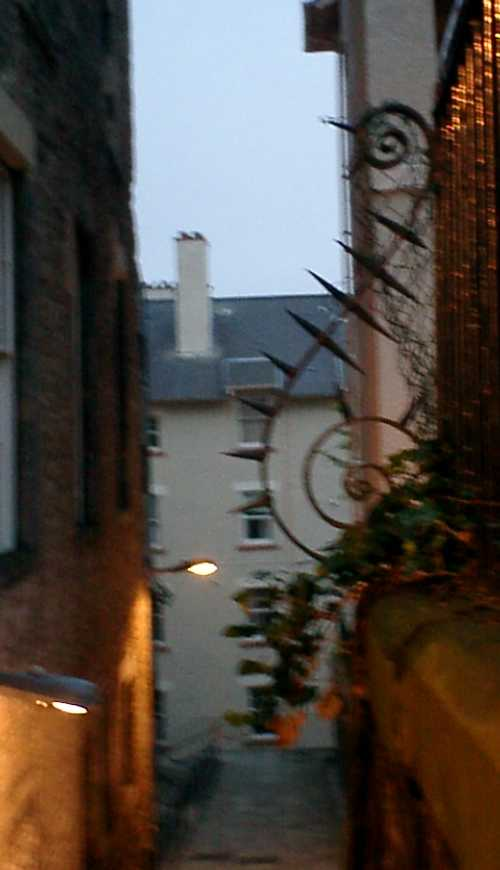
\includegraphics[width=1\hsize]{image200707/gurutitle.jpg}
\end{minipage}
\begin{minipage}{0.39\hsize}
 {\Huge #1
 }
\end{minipage}
\end{frame}
}

\begin{document}
\frame{\titlepage{}}

\section{Intro}

\emtext{Agenda}

\section{}
\begin{frame}
 \frametitle{Agenda}
  \begin{itemize}
  \item $B:#2s$NL\E*H/I=(B
  \item Debian Package $B$r:n@.$9$kA0$N=`Hw(B
  \item $B:#2s$N@8lS(B
  \item $B%W%m%0%i%`$,F0:n$r3NG'$9$k(B
  \item Debian Package $B$N?w7A$r:n$k(B
  \item debian/control $B%U%!%$%k$NJT=8(B
  \item debian/changelog $B%U%!%$%k$NJT=8(B
  \item debian/copyright $B%U%!%$%k$NJT=8(B
  \item debian/rules $B%U%!%$%k$rJT=8$9$k(B
  \item Debian Package$B!!$N:n@.(B
  \item Debian Package $B$N%F%9%H(B
  \item $BK\F|$N$^$H$a(B
  \item $B=*$o$j$K(B
  \item $B<A5?1~Ez(B
 \end{itemize}
\end{frame}

\section{$B:#2s$NL\E*(B}
\emtext{$B:#2s$NL\E*(B}

\begin{frame}
\alert{{\LARGE$B!!%7%s%0%k%P%$%J%j$N(B Debian Package $B$,:n@.$G$-$k$h$&$K$J$k$3$H!#(B}}
\end{frame}

\section{Debian Package $B$r:n@.$9$kA0$N=`Hw(B}
\emtext{Debian Package $B$r:n@.$9$kA0$N=`Hw(B}

\section{Debian Package $B:n@.4D6-(B}
\begin{frame}
$B0J2<$N4D6-JQ?t$r@_Dj$7$F$*$/$HJXMx!#(B

\begin{itemize}
  \item DEBFULLNAME $B$N@_Dj(B

    Debian Package $B$N%a%s%F%JL>(B
  \item DEBEMAIL $B$N@_Dj(B

    Debain Package  $B%a%s%F%J%s%9MQ$N%a!<%k%"%I%l%9(B
\end{itemize}
\end{frame}

\begin{frame}[containsverbatim]

\begin{commandline}
$ cat ~/.bashrc
--$BN,(B--
export DEBFULLNAME="Nobuhiro Iwamatsu"
export DEBEMAIL=iwamatsu@nigauri.org
--$BN,(B--
$ source ~/.bashrc
\end{commandline}
\end{frame}

\begin{frame}{$BI,MW$J%Q%C%1!<%8(B}
$B:GDc8BI,MW$JI,MW$J%Q%C%1!<%8$O0J2<$NDL$j!#(B
\begin{itemize}
 \item devscripts
 \item debhelper
 \item lintian/linda
 \item gcc 
 \item binutils 
 \item libc6-dev
 \item dh-make
\end{itemize}

$B$"$k$HJXMx$J%Q%C%1!<%8(B
\begin{itemize}
\item apt-file
\item pbuilder
\end{itemize}
\end{frame}

\section{$B:#2s$N@8lS(B}
\emtext{$B:#2s$N@8lS(B}

\begin{frame}[containsverbatim]
{\LARGE sl}
\begin{commandline}


      ====        ________                ___________
  _D _|  |_______/        \__I_I_____===__|_________|
   |(_)---  |   H\________/ |   |        =|___ ___|      _________________ 
   /     |  |   H  |  |     |   |         ||_| |_||     _|                \_____A
  |      |  |   H  |__--------------------| [___] |   =|                        |
  | ________|___H__/__|_____/[][]~\_______|       |   -|                        |
  |/ |   |-----------I_____I [][] []  D   |=======|____|________________________|_
__/ =| o |=-~~\  /~~\  /~~\  /~~\ ____Y___________|__|__________________________|_
 |/-=|___||    ||    ||    ||    |_____/~\___/          |_D__D__D_|  |_D__D__D_|
  \_/      \__/  \__/  \__/  \__/      \_/               \_/   \_/    \_/   \_/

\end{commandline}
\end{frame}

\section{$B%W%m%0%i%`$,F0:n$r3NG'$9$k(B}
\emtext{$B%W%m%0%i%`$,F0:n$r3NG'$9$k(B}

\begin{frame}[containsverbatim]
$B$^$:!"%W%m%0%i%`$,F0:n$9$k$+3NG'$7$^$7$g$&!#(B
\begin{commandline}
$ tar -xf sl.tar
$ cd sl
$ make
\end{commandline}
\end{frame}

\begin{frame}[containsverbatim]
curses.h $B$,$J$$$?$a!"%3%s%Q%$%k$K<:GT$7$^$7$?!#(B
\begin{commandline}
$ tar -xf sl.tar
$ cd sl
$ make
 make
cc -O -o sl sl.c -lcurses -ltermcap
sl.c:30:20: error: curses.h: No such file or directory
sl.c: In function 'my_mvaddstr':
sl.c:42: error: 'ERR' undeclared (first use in this function)
sl.c:42: error: (Each undeclared identifier is reported only once
........ 
\end{commandline}
\end{frame}

\begin{frame}[containsverbatim]
curses.h $B$r;}$C$?(B Debian Package $B$,I,MW$G$9!#(B
$B$I$N%U%!%$%k$,$I$N%Q%C%1!<%8$8$h$C$F%$%s%9%H!<%k$5$l$k$N$+!"D4$Y$k$K$O(B
\alert{apt-file}$B$r;H$&$HJXMx$G$9!#(B
\begin{commandline}
# sudo apt-file update
$ apt-file search /usr/include/curses.h
libncurses5-dev: usr/include/curses.h
\end{commandline}
\end{frame}

\begin{frame}[containsverbatim]
\alert{libncueses5-dev} $B%Q%C%1!<%8$r%$%s%9%H!<%k$7$F:FEY%3%s%Q%$%k$7$^$7$g$&!#(B
\begin{commandline}
# apt-get update
# apt-get install libncurses5-dev
$ make
 make
cc -O -o sl sl.c -lcurses -ltermcap
.......
\end{commandline}
\end{frame}

\begin{frame}[containsverbatim]
$B%3%s%Q%$%k$,DL$C$?$N$G!"F0:n%F%9%H$r$7$^$7$g$&!#(B
\begin{commandline}
% ./sl
\end{commandline}
\end{frame}

\section{Debian Package $B$N?w7A$r:n$k(B}
\emtext{Debian Package $B$N?w7A$r:n$k(B}

\begin{frame}[containsverbatim]
$B%G%#%l%/%H%j$K%P!<%8%g%s$,$J$$>l9g$O%P!<%8%g%s$,IU$$$?%G%#%l%/%H%jL>$KJQ99$7$^$9!#(B
Debian Package $B$N?w7A$r:n@.$9$k$K$O!"(Bdh\_make $B%3%^%s%I$r;H$$$^$9!#(B

%Debian Package $B$O%Q%C%1!<%8$N%P!<%8%g%s$rMW5a$7$^$9!#%G%#%l%/%H%j$K%P!<%8%g%s$,(B
%$B$J$$>l9g$O%P!<%8%g%s$,IU$$$?%G%#%l%/%H%jL>$KJQ99$7$^$9!#(B
\begin{commandline}
$ tar -xf sl.tar
$ mv sl sl-0.0.0
$ cd sl-0.0.0
$ dh_make 
\end{commandline}
\end{frame}

\begin{frame}[containsverbatim]
\begin{commandline}
iwamatsu@chimagu:~/sl-0.0.0$ dh_make

Type of package: single binary, multiple binary, 
library, kernel module or cdbs?
 [s/m/l/k/b] 
\end{commandline}
\end{frame}

\begin{frame}
\begin{itemize}
  \item s: $B0l$D$N<B9T%P%$%J%j$rDs6!$9$k%Q%C%1!<%8(B
  \item m: 2$B$D0J>e$N<B9T%P%$%J%j$rDs6!$9$k%Q%C%1!<%8(B
  \item l: $B%i%$%V%i%jMQ%Q%C%1!<%8(B
  \item k: $B%+!<%M%k%b%8%e!<%kMQ%Q%C%1!<%8(B
  \item b: cdbs $B$r;H$C$?%Q%C%1!<%8(B
\end{itemize}
\end{frame}

\begin{frame}[containsverbatim]
\begin{commandline}
$ dh_make

Type of package: single binary, multiple binary, 
library, kernel module or cdbs?
 [s/m/l/k/b] s
Maintainer name : Nobuhiro Iwamatsu
Email-Address   : iwamatsu@nigauri.org 
Date            : Thu, 21 Feb 2008 15:46:57 +0900
Package Name    : sl
Version         : 0.0.0
License         : blank
Type of Package : Single
Hit <enter> to confirm:
\end{commandline}
\end{frame}

\begin{frame}[containsverbatim]
\begin{commandline}
$ dh_make

Type of package: single binary, multiple binary, 
library, kernel module or cdbs?
 [s/m/l/k/b] s
Maintainer name : Nobuhiro Iwamatsu
Email-Address   : iwamatsu@nigauri.org 
Date            : Thu, 21 Feb 2008 15:46:57 +0900
Package Name    : sl
Version         : 0.0.0
License         : blank
Type of Package : Single
Hit <enter> to confirm:
 
Could not find sl_0.0.0.orig.tar.gz
Either specify an alternate file to use with -f,
or add --createorig to create one.
\end{commandline}
\end{frame}

\begin{frame}[containsverbatim]
xxx.orig.tar.gz $B$,$J$$$H!"%(%i!<$K$J$j$^$9!#(B\\
--createorig $B%*%W%7%g%s$r2C$($F!!(Bdh\_make$B$r<B9T$7$^$7$g$&!#(B

\begin{commandline}
$ dh_make --createorig
\end{commandline} 
\end{frame}

\section{}

\begin{frame}[containsverbatim]

dh\_make $B<B9T8e!"(Bdebian $B%G%#%l%/%H%j$,:n@.$5$l$^$9!#(B
\begin{commandline}
$ ls ./debian/
README.Debian  control    dirs  emacsen-remove.ex   
init.d.lsb.ex  manpage.xml.ex   mogeri.doc-base.EX  
preinst.ex     watch.ex$B!!!!(Bchangelog  copyright  
docs           emacsen-startup.ex manpage.1.ex     
menu.ex        postinst.ex      prerm.ex
compat         cron.d.ex        emacsen-install.ex  
init.d.ex      manpage.sgml.ex  sl-default.ex  
postrm.ex      rules
\end{commandline}
\end{frame}

\begin{frame}[containsverbatim]
*.ex / *.EX $B$O%5%s%W%k$J$N$G:o=|$7$^$9!#(B
\begin{commandline}
$ rm -rf ./debian/*.ex
$ rm -rf ./debian/*.EX
\end{commandline}
\end{frame}

\begin{frame}[containsverbatim]

$B:GDc8BI,MW$J(B debian $B%G%#%l%/%H%j0J2<$K$"$k%U%!%$%k$O0J2<$NDL$j$G$9!#!#(B

\begin{itemize}
  \item README.Debian --$B!!(BPackage $B$N(BREADME
  \item control       -- Package $B$N@bL@!"%S%k%I$KI,MW$J>pJs$J$I(B
  \item dirs          -- Package $B$GMxMQ$9$k%G%#%l%/%H%j$r5-=R(B
  \item changelog     -- Package $B$NJQ99MzNr(B
  \item copyright     -- Package $B$N%3%T!<%i%$%H(B
  \item docs          -- $B%I%-%e%a%s%H%U%!%$%k0lMw(B
  \item rules         -- Package $B:n@.MQ$N%9%/%j%W%H(B(Makefile)
  \item compat        -- debhelper $B$N%P!<%8%g%s(B
\end{itemize}
\end{frame}

\section{debian/control $B%U%!%$%k$NJT=8(B}
\emtext{debian/control $B%U%!%$%k$NJT=8(B}

\begin{frame}[containsverbatim]
\begin{commandline}
Source: sl
Section: game
Priority: extra
Maintainer: Nobuhiro Iwamatsu <iwamatsu@nigauri.org>
Build-Depends: debhelper (>= 5),libncurses5-dev
Standards-Version: 3.7.2

Package: sl
Architecture: any
Depends: ${shlibs:Depends}, ${misc:Depends}
Description: Key type correction software
 Key type correction software for 'ls' command.
\end{commandline}
\end{frame}

\section{debian/changelog $B%U%!%$%k$NJT=8(B}
\emtext{debian/changelog $B%U%!%$%k$NJT=8(B}

\begin{frame}[containsverbatim]

$B<!$K(B Debian $B$N(B Changelog $B$rJT=8$7$^$7$g$&!#(B
$BJT=8$9$k$K$O!"(Bdch $B%3%^%s%I$r;H$$$^$9!#(B

\begin{commandline}
$ dch 
sl (0.0.0-1) unstable; urgency=low

  * Initial release

 -- Nobuhiro Iwamatsu <iwamatsu@nigauri.org> \
     Sun, 24 Feb 2008 01:01:53 +0900

\end{commandline}
\end{frame}

\section{debian/copyright $B%U%!%$%k$NJT=8(B}
\emtext{debian/copyright $B%U%!%$%k$NJT=8(B}

\begin{frame}[containsverbatim]
\begin{commandlinesmall}
This package was debianized by \ 
Nobuhiro Iwamatsu <iwamatsu@nigauri.org> on
Thu, 21 Feb 2008 16:13:47 +0900.

It was downloaded from http://www.is.titech.ac.jp/~toyoda/

Upstream Author:
 Toyoda Masashi <toyoda@is.titech.ac.jp>

Copyright:

 Copyright 1993,1998 Toyoda Masashi (toyoda@is.titech.ac.jp)

License:
 Everyone is permitted to do anything on this program 
 including copying,
 modifying, and improving, unless you try to pretend that 
 you wrote it.
 i.e., the above copyright notice has to appear in all copies.
 THE AUTHOR DISCLAIMS ANY RESPONSIBILITY WITH REGARD TO 
 THIS SOFTWARE.

The Debian packaging is \
(C) 2008, Nobuhiro Iwamatsu <iwamatsu@nigauri.org> and
is licensed under the GPL, see `/usr/share/common-licenses/GPL'.

# Please also look if there are files or directories which have a
# different copyright/license attached and list them here.
\end{commandlinesmall}
\end{frame}

\begin{frame}
$B$a$s$I$/$5$$$N$G!"%3%T!<!#(B
\end{frame}

\begin{frame}
$B<B:]$O!"%=%U%H%&%'%"$NCx:n8"$r;}$C$F$$$k?M$KO"Mm$r$H$j!"%i%$%;%s%9$r3NG'$9$kI,MW$,$"$j$^$9!#(B
\end{frame}

\section{debian/rules $B%U%!%$%k$rJT=8$9$k(B}
\emtext{debian/rules $B%U%!%$%k$rJT=8$9$k(B}
\begin{frame}[containsverbatim]
debian/rules $B$O!!(BDebian Package $B$r:n@.$9$k(B Makefile $B$G$9!#(B
\begin{itemize}
 \item configure $B%?!<%2%C%H(B
 \item build $B%?!<%2%C%H(B
 \item clean $B%?!<%2%C%H(B
 \item install $B%?!<%2%C%H(B
\end{itemize}
\end{frame}

\begin{frame}[containsverbatim]
$B:#2s$O%7%s%W%k$J%W%m%0%i%`$J$N$G!"JQ99$9$kI,MW$O$"$j$^$;$s!#(B
\end{frame}

\section{$B$H$j$"$($:(B Package $B$r:n@.$9$k(B}
\emtext{$B$H$j$"$($:(B Package $B$r:n@.$9$k(B}
\begin{frame}[containsverbatim]

Debian Package $B$r:n$k;~$O!"(B\alert{debuild} $B%3%^%s%I$r;H$$$^$9!#(B
\begin{commandline}
$ debuild -us -uc
\end{commandline}
-us $B%=!<%9%Q%C%1!<%8$K(BGPG$B%5%$%s$r$7$J$$(B

-uc *.changes $B%U%!%$%k$K(B GPG $B%5%$%s$r$7$J$$(B

\end{frame}

\begin{frame}[containsverbatim]
\begin{commandline}
$ debuild -us -uc
 fakeroot debian/rules clean
dh_testdir
dh_testroot
rm -f build-stamp configure-stamp
# Add here commands to clean up after the \
build process.
/usr/bin/make clean
make[1]: $B%G%#%l%/%H%j(B `/tmp/sl-0.0.0' $B$KF~$j$^$9(B
make[1]: *** $B%?!<%2%C%H(B `clean' $B$r(B make $B$9$k%k!<%k(B \
$B$,$"$j$^$;$s(B.  $BCf;_(B.
make[1]: $B%G%#%l%/%H%j(B `/tmp/sl-0.0.0' $B$+$i=P$^$9(B
make: *** [clean] $B%(%i!<(B 2
debuild: fatal error at line 1239:
fakeroot debian/rules clean failed
\end{commandline}
\end{frame}

\section{Makefile $B$N=$@5(B}
\emtext{Makefile $B$N=$@5(B}
\begin{frame}[containsverbatim]

$B?^(Brules $B%U%!%$%k$H(BMakefile $B$N4X78?^(B
$B:#$N(BMakefile
\begin{commandline}
CC=cc
CFLAGS=-O

sl: sl.c sl.h
  $(CC) $(CFLAGS) -o sl sl.c -lcurses -ltermcap
# $(CC) $(CFLAGS) -o sl sl.c -lcurses
\end{commandline}
\end{frame}

\begin{frame}[containsverbatim]
$B=$@58e(B
\begin{commandline}
CC=cc
CFLAGS=-O
BINDIR?=/usr/games/ <--- $B%$%s%9%H!<%k@h$rDI2C(B

\end{commandline}
\alert{BINDIR} : $B<B9T%P%$%J%j$,%$%s%9%H!<%k$5$l$k%G%#%l%/%H%j(B
\end{frame}

\begin{frame}[containsverbatim]
$B=$@58e(B
\begin{commandline}

install:  <-- install $B%?!<%2%C%H$rDI2C(B
  install -d ${DESTDIR}${BINDIR}
  install -m 755 sl ${DESTDIR}${BINDIR}

clean:    <-- clean $B%?!<%2%C%H$rDI2C(B
  rm -rf sl

\end{commandline}
\alert{DESTDIR}: Debian Package $B$N%$%s%9%H!<%k$5$l$k(B TOP $B%G%#%l%/%H%j(B
\end{frame}

\section{$B:FEY(BDebian Package$B$r:n@.(B}
\emtext{$B:FEY(BDebian Package$B$r:n@.(B}
\begin{frame}[containsverbatim]
\begin{commandline}
$ debuild -us -uc
......
dh_shlibdeps
dh_gencontrol
dpkg-gencontrol: warning: unknown substitution variable ${misc:Depends}
dh_md5sums
dh_builddeb
dpkg-deb: building package `sl' in `../sl_0.0.0-1_i386.deb'.
 dpkg-genchanges
dpkg-genchanges: including full source code in upload
dpkg-buildpackage (debuild emulation): full upload (original source is included)
Now running lintian...
W: sl: binary-without-manpage sl
Finished running lintian.
\end{commandline}
\end{frame}

\section{Debian Package$B$N%F%9%H(B}
\emtext{Debian Package $B$N%F%9%H(B}

\section{}
\begin{frame}[containsverbatim]
\begin{itemize}
  \item pbuilder

   $B:GDc8B$N(BDebian system$B$+$i!"%Q%C%1!<%8$r:n@.$9$k$?$a$N%D!<%k!#(B 

$B!!!!!!(B\begin{commandline}
$ sudo /usr/sbin/pbuilder build sl_0.0.0-1.dsc 
   \end{commandline}
  \item piuparts 

   Debian Package $B$N(B $B%$%s%9%H!<%k(B/$B%"%s%$%s%9%H!<%k$N%A%'%C%/$r$9$k$?$a$N%D!<%k!#(B

\end{itemize}
\end{frame}

\section{$B$^$H$a(B}
\emtext{$BK\F|$N$^$H$a(B}

\section{}
\begin{frame}
\begin{itemize}
  \item $B$^$:$O!"%=%U%H%&%'%"$,F0:n$9$k$+3NG'$9$k(B
  \item dh\_make $B%3%^%s%I(B $B$G%Q%C%1!<%8$N?w7A$r:n@.$9$k(B
  \item debuild $B%3%^%s%I(B $B$G%Q%C%1!<%8:n@.(B
  \item $B%i%$%;%s%9$d%3%T!<%i%$%H$N3NG'$r$9$k$3$H(B
  \item lintian/linda $B$G(B $B%Q%C%1!<%8$N%A%'%C%/(B
  \item $B%$%s%9%H!<%k$7$FF0:n3NG'$^$G9T$&(B
  \item $B%"%s%$%s%9%H!<%k$N3NG'$bK:$l$:$K(B
\end{itemize}
\end{frame}

\section{$B>pJs8;(B}
\emtext{$B>pJs8;(B}
\begin{frame}
\begin{itemize}
  \item Debian Project / Debian JP Project Website

    \url{http://www.debain.org}

    \url{http://www.debain.or.jp}

  \item $BEl5~%(%j%"(BDebian$BJY6/2q(B

    \url{http://tokyodebian.alioth.debian.org}
  \item Debian Policy
    
    \url{http://www.debian.org/doc/debian-policy/}

  \item Debian $B?7%a%s%F%J%,%$%I(B
    
    \url{http://www.debian.org/doc/manuals/maint-guide/index.ja.html}
\end{itemize}
\end{frame}

\section{$B=*$o$j$K(B}
\emtext{$B=*$o$j$K(B}

\section{}
\begin{frame}
$B:#G/$N(BDebian$BJY6/2q$G$O!"Kh7nMM!9$J(BDebian Pakcage $B$N(B
$B:n@.J}K!$r$_$J$5$s$KEA<x$7$^$9!#(B
\begin{itemize}
  \item $B%G!<%?$@$1$N(BDebianPackage$B:n@.J}K!(B
  \item VCS$B$r;H$C$?(BDebian Package$B$N:n@.J}K!(B
  \item $B%i%$%V%i%j$N(BDebian Package $B:n@.J}K!(B
  \item $B$J$I$J$I(B
\end{itemize}
\end{frame}


\section{$B<A5?1~Ez(B}
\emtext{$B<A5?1~Ez(B}

\end{document}

;;; Local Variables: ***
;;; outline-regexp: "\\([ 	]*\\\\\\(documentstyle\\|documentclass\\|emtext\\|section\\|begin{frame}\\)\\*?[ 	]*[[{]\\|[]+\\)" ***
;;; End: ***
